\documentclass[pdftex,12pt,letter]{article}
\usepackage{fancyhdr}
\usepackage{enumerate}
\usepackage{tabularx}
\usepackage{graphicx}
\usepackage{array}
\usepackage[justification=justified,singlelinecheck=false]{caption}
\usepackage{placeins}
\pagestyle{fancy}
\makeatletter
  \renewcommand\@seccntformat[1]{\csname the#1\endcsname.\quad}
\makeatother

\newcolumntype {Y}{ >{\raggedright \arraybackslash }X}
\newcommand{\HRule}{\rule{\linewidth}{0.5mm}}
\captionsetup{labelformat=empty}

\begin{document}

\begin{titlepage}
\begin{flushright}
\HRule \\[0.4cm]
{ \bfseries
{\huge Software Requirements Specification\\[1cm]}
{\Large for\\[1cm]}
{\huge CWRUtility\large{\footnote[1]{Working title}}\\[4cm]}
{\large Prepared by\\Jason Kuster, Stuart Long, and William Ordivay\\[1cm]
Version 1.0\\[1cm]
KOALAA Development\\[1cm]
October 1, 2012}}
\end{flushright}
\end{titlepage}
\tableofcontents{}
\vspace{5cm}
\begin{table}[h]
\caption*{\bfseries Revision History}
\begin{tabularx}{\textwidth }[t]{|l|Y|Y|Y|}
\hline
\bfseries Name & \bfseries Date & \bfseries Reasons for Change & \bfseries Version \\ \hline
Kuster, Long, Ordiway & 9/22/2012 & Initial Draft & 1.0 draft 1\\ \hline
\end{tabularx}
\end{table}
\newpage
\section{Introduction}
\subsection{Purpose}
This Software Requirements Specification describes the software functional and nonfunctional requirements for release 1.0 of CWRUtility. This specification document is intended for the solu use of the members of the project team that will implement and verify the correction functioning of the system. Unless otherwise specified, all requirements documented here are high priority and committed for release 1.0. 

\subsection{Project Scope and Product Features}
CWRUtility will allow CWRU students, faculty, and staff to easily access CWRU services and information in an easy-to-use way. A detailed project description is available in the \emph{CWRUTility Vision and Scope Document}[1]. The section in that document titled "Scope of initial and subsequent releases" lists the features that are scheduled for full or partial implementation in this release.

\subsection{References}
\begin{enumerate}[1.]
\item Kuster et al. \emph{Vision and Scope Document for CWRUtility}, https://github\\.com/jasonkuster/EECS-393/blob/master/V%26S/VisionAndScope.pdf
\end{enumerate}

\section{Overall Description}
\subsection{Product Perspective}
CWRUtility is a new system that replaces the need for cumbersome navigation of all of the CWRU services in favor of a streamlined and custom-built mobile experience. The context diagram in Figure 1 illustrates the external entities and system interfaces for release 1.0. The system is expected to evolve over two releases, ultimately encompassing all of the services CWRU students, faculty, and staff use every day.
\subsection{User Classes and Characteristics}
\noindent Users: CWRUtility users are CWRU students, faculty, or staff members who wish to use our app in order to access CWRU services. The number of people at CWRU who possess Windows Phone 7/8 devices is is unknown, but can be estimated in the area of 200 to 400 assuming that about half to 3/4 of the community possesses smartphones and the current figures put Windows Phone's marketshare at 3.5\%. Our app will probably be used daily by 75\% of installed users.\\\\
CWRU Services:  The CWRU services are the services enumerated in Diagram 1 with which CWRUtility will have active communication. These services will be accessed several times per day by each instance of the application as it pulls data from the background. Multiple users may access the same service at the same time. Downtime in a service will result in downtime for the application.
\begin{figure}[h]
\begin{center}
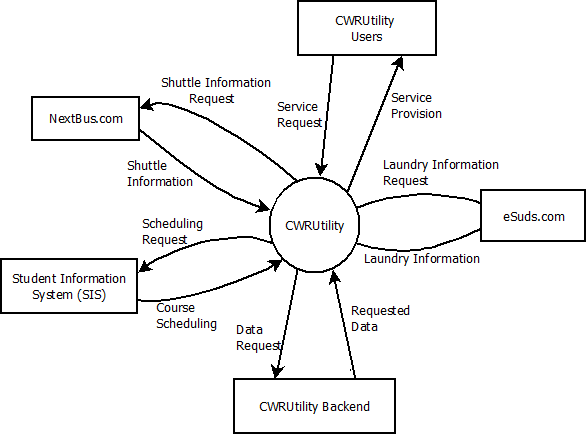
\includegraphics[width=110mm]{ContextDiagram.png}\\
\caption{Figure 1: \emph{Context diagram for release 1.0 of CWRUtility}}
\end{center}
\end{figure}
\subsection{Operating Environment}
\begin{enumerate}[{O}E-1:]
\item CWRUtility shall operate on the Windows Phone 7 and Windows Phone 8 operating systems.
\end{enumerate}
\subsection{Design and Implementation Constraints}
\begin{enumerate}[CO-1:]
\item Design, code, and maintenance will conform to KOALAA's coding and documentation standards.
\item All user interfaces will be laid out with XAML.
\item All code will be written in C\#.
\end{enumerate}
\subsection{User Documentation}
\begin{enumerate}[UD-1:]
\item System shall provide in-system tutorial and help documentation accessible via an easy to find button.
\end{enumerate}
\subsection{Assumptions and Dependencies}
\begin{enumerate}[{A}S-1:]
\item User's Windows Phone 7/8 device is equipped with an internet connection.
\end{enumerate}
\begin{enumerate}[DE-1:]
\item This application depends on the continuing functionality of the connected services (e.g. NextBus.com, eSuds.com, and SIS)
\end{enumerate}
\section{System Features}
\subsection{Schedule Courses}
\subsubsection{Description and Priority}
A CWRUtility User may search for CWRU courses by semester and course name. Duplicate courses in a semester are returned as a drop down list. The User may then choose to add that course to his or her current schedule. Information for CWRU courses are pulled from the Student Information System Service. The User may also delete courses from his or her current schedule. The system displays the User's schedule in a standard calendar format. Priority: High
\subsubsection{Stimulus/Response Sequences}
\begin{description}\itemsep1pt
\item[Stimulus:] User switches to this feature.
\item[Response:] System displays user's current schedule.
\item[Stimulus:] User searches for a course with a specified semester and course.
\item[Response:] System queries SIS for detailed course information and relays it to user. If more than one course match the given semester and course name, results are displayed in a dropdown list.
\item[Stimulus:] User adds chosen course to schedule
\item[Response:] System plots course on user's current schedule.
\item[Stimulus:] User selects a course to remove from schedule.
\item[Response:] System removes selected course from schedule.
\end{description}
\subsubsection{Functional Requirements}
\begin{table}[!h]
\begin{tabularx}{\textwidth }[t]{|l Y|}
\hline
~&~\\
Courses.Search & The system will allow the user to search for a course based on user inputted course name and semester.\\ 
~&~\\
Courses.Search.Invalid & If the user enters an invalid course name or semester, no course will be returned by the system and it will inform the user appropriately.\\
~&~\\
Courses.Search.Return & If a course is found that matches the user criteria, the system shows the course and its information. \\
~&~\\
Courses.Search.Multiple & If more than one course matches the user criteria, the system will display the courses in a drop-down list that allows the user to select an appropriate course.\\
~&~\\
\hline
\end{tabularx}
\end{table}
\begin{table}[!h]
\begin{tabularx}{\textwidth }[t]{|l Y|}
\hline
~&~\\
Courses.Schedule & The system will display user added courses on a calendar formatted schedule.\\
~&~\\
Courses.Schedule.Add & Courses selected to be added to the schedule will be added to the schedule and placed in their appropriate time slot.\\
~&~\\
Courses.Schedule.Remove & The system will allow users to remove any and all courses from the user's schedule.\\
~&~\\
\hline
\end{tabularx}
\end{table}
\FloatBarrier
\subsection{Map}
\subsubsection{Description and Priority}
All relevant campus buildings should be accurately labelled on the map. This includes not only academic buildings but residence halls, cafeterias, and other miscellaneous CWRU-owned buildings as well.\\
Upon being opened, if the user has entered in courses, the map should predict their next destination and offer a map perspective encompassing both their current location and their projected next location.\\
The map will offer the student the ability to navigate from their current location to their next class, or to an alternate location.
\subsubsection{Stimulus/Response Sequences}
Stimulus: User opens map.\\
Response: App queries its stored information regarding whether the student has a class, then sets the starting map coordinates and zoom level accordingly.\\
Stimulus: User requests directions.\\
Response: Map provides directions from the user's current location to the specified location.\\
\subsubsection{Functional Requirements}
\subsection{Nextbus}
\subsubsection{Description and Priority}
A user will be presented with the Case Western University nextbus webpage which presents an active timer until busses arrive. Users can specify which bus route, which stop, and which direction 
\subsection{Directory}
\subsubsection{Description and Priority}
The system will include a directory that lists hours, location, and phone numbers of campus resources. The user will be able to browse the directory and select a resource to see the above information about it. The directory will be designed such that more resources can be added easily. Priority: medium.
\subsubsection{Stimulus/Response Sequences}
\begin{description}\itemsep1pt
\item[Stimulus:] User switches to directory feature.
\item[Response:] System displays list of CWRU services in the directory.
\item[Stimulus:] Users selects a service from the directory.
\item[Response:] System queries its own database/backend and displays the stored information about that service to the user.
\item[Stimulus:] Users clicks on a the phone number of some selected service
\item[Response:] System attempts to place a mobile phone call using selected phone number
\end{description}
\subsubsection{Functional Requirements}
\begin{table}[!h]
\begin{tabularx}{\textwidth }[t]{|l Y|}
\hline
~&~\\
Directory.Browse & The system will allow the user to browse through CWRU services\\ 
~&~\\
Directory.Browse.Select & If the user selects a service from the directory, system displays descriptive information about the service, e.g. hours. location, and phone number.\\
~&~\\
\hline
\end{tabularx}
\end{table}
\begin{table}[!h]
\begin{tabularx}{\textwidth }[t]{|l Y|}
\hline
~&~\\
Directory.Call & After selecting the service, if the user clicks that service's phone number, the cell phone the system is implemented dials that phone number\\
~&~\\
\hline
\end{tabularx}
\end{table}
\FloatBarrier
\subsection{Menu}
\subsubsection{Description and Priority}
The system will display the semester menu's for both major campus dining halls, Fribley Dining Hall and Leutner Dining Hall. The system will layout of the menus in a tabular format, so at anytime the menu portion of the application will either display the Leutner menu or the Fribley menu, depending on which dining is selected. Priority: low
\subsubsection{Stimulus/Response Sequences}
\begin{description}\itemsep1pt
\item[Stimulus:] User switches to this feature.
\item[Response:] System displays last menu user viewed, or a default menu if first use.
\item[Stimulus:] User selects a dining hall whose menu the user wants to view.
\item[Response:] The system displays the menu for the specified dining hall.
\end{description}
\subsubsection{Functional Requirements}
\begin{table}[!h]
\begin{tabularx}{\textwidth }[t]{|l Y|}
\hline
~&~\\
Menu.Display & System will display the menu for a selected campus dining hall.\\ 
~&~\\
Menu.Display.Select & System will switch displayed menu based on which tab is selected. \emph{The Case Daily}\\
~&~\\
\hline
\end{tabularx}
\end{table}
\FloatBarrier
\subsection{Case News}
\subsubsection{Description and Priority}
The system will list recent news from CWRU and allow the user to select a news story to discover more information about it. The two main sources for these stories will be the \emph{The Case Daily} and \emph{The Observer}. Priority: low.
\subsubsection{Stimulus/Response Sequences}
\begin{description}\itemsep1pt
\item[Stimulus:] User switches to this feature.
\item[Response:] System displays a list of clickable panels that display the title and source of a news story.
\item[Stimulus:] User selects a news story from the list.
\item[Response:] System switches to a new window that displays the article or story in full.
\end{description}
\subsubsection{Functional Requirements}
\begin{table}[!h]
\begin{tabularx}{\textwidth}[t]{|l Y|}
\hline
~&~\\
News.Display & System displays the list of current news.\\
~&~\\
News.Display.Story & Stories are displayed as panels that show their title and source.\\
~&~\\
News.Display.Update & The list of stories are updated daily to reflect new stories from either \emph{The Observer} or \emph{The Case Daily}.\\
~&~\\
\hline
\end{tabularx}
\end{table}
\begin{table}[!h]
\begin{tabularx}{\textwidth}[t]{|l Y|}
\hline
~&~\\
News.Story & If a user selects a story from the list, a new window appears that displays detailed information about the story.\\
~&~\\
News.Story.Query & To obtain information for a specific story, the system queries the corresponding source.\\
~&~\\
\hline
\end{tabularx}
\end{table}
\FloatBarrier
\subsection{eSuds}
\subsubsection{Description and Priority}
The system will allow the user to view laundry information for all of the residence halls at CWRU. The user will select a residence hall from a list to view that hall's specific laundry information. Priority: medium
\subsubsection{Stimulus/Response Sequences}
\begin{description}\itemsep1pt
\item[Stimulus:] User switches to this feature.
\item[Response:] System displays the laundry information for the user's last selected residence hall. If this is the first time the user has used the eSuds feature, a default residence hall will be displayed.
\item[Stimulus:] User selects a residence hall from a drop down list.
\item[Response:] The system will update the current laundry information with the laundry information for the selected residence hall.
\end{description}
\subsubsection{Functional Requirements}
\begin{table}[!h]
\begin{tabularx}{\textwidth}[t]{|l Y|}
\hline
~&~\\
eSuds.Display & System displays laundry information and a drop-down list of CWRU residence halls.\\ 
~&~\\
eSuds.Display.Laundry & Laundry information includes numbers of washers, dryers, and how much time is remaining on each of the different machines \\
~&~\\
eSuds.Display.DropDown & On the eSuds display there will be a dropdown menu that allows the user to select different CWRU residence halls.\\
~&~\\
\hline
\end{tabularx}
\end{table}
\begin{table}[!h]
\begin{tabularx}{\textwidth}[t]{|l Y|}
\hline
~&~\\
eSuds.Connection & System maintains a constant connection to the eSuds.com webservice in order to provide up-to-date information on laundry.\\
~&~\\
\hline
\end{tabularx}
\end{table}
\FloatBarrier
\subsection{5YearCal}
\subsubsection{Description and Priority}
The system will display the current CWRU 5-year academic calendar as provided by the university. The system will query the CWRU official website at the beginning of every Fall term to obtain the latest edition of the calendar. Priority: low.
\subsubsection{Stimulus/Response Sequences}
\begin{description}\itemsep1pt
\item[Stimulus:] User switches to this feature.
\item[Response:] System displays the current 5-year academic calendar.
\item[Stimulus:] Fall semester begins.
\item[Response:] System queries the CWRU website for the most up-to-date calendar.
\end{description}
\subsubsection{Functional Requirements}
\begin{table}[!h]
\begin{tabularx}{\textwidth}[t]{|l Y|}
\hline
~&~\\
5YearCal.Display & System displays the current CWRU 5-year academic calendar\\ 
~&~\\
5YearCal.Display.Update & At the beginning of each Fall semester, the system will obtain the most recent 5-year academic calendar from the CWRU website.\\
~&~\\
\hline
\end{tabularx}
\end{table}
\FloatBarrier
\section{External Interface Requirements}
\subsection{User Interfaces}
\begin{enumerate}[UI-1:]
\item The user interface will comprise of a separate page for each feature provided by the system, with the title of the feature at the top of the page and the content of the page underneath it.
\item The user interface will conform to Windows Phone application standards.
\end{enumerate}
\subsection{Hardware Interfaces}
\begin{enumerate}[HI-1:]
\item System will be accessed and interacted with via a Windows Phone 7 or Windows Phone 8 mobile device.
\end{enumerate}
\subsection{Software Interfaces}
TBD
\subsection{Communication Interfaces}
\begin{enumerate}[CI-1]
\item Upon user request, the system will use the user's phone to place a phone call to the number selected by the user.
\end{enumerate}
\section{Other Nonfunctional Requirements}
\subsection{Performance Requirements}
\begin{enumerate}[PR-1:]
\item Information requested by the user shall be returned and displayed on the screen after no more than 1 second.
\item System will occupy no more than 256MB on user's phone.
\end{enumerate}
\subsection{Reliability Requirements}
\begin{enumerate}[RR-1:]
\item No more than 1 crash is 1000 application instances
\item Updates will be backwards compatible, i.e. they will not break any functionality.
\end{enumerate}
\subsection{Safety Requirements}
\begin{enumerate}[SR-1:]
\item Important information (e.g. phone number for Case Security) must always be up-to-date and accurate.
\end{enumerate}
\subsection{Security Requirements}
No security requirements have been identified.
\subsection{Software Quality Attributes}

\section*{Appendix A: Data Dictionary and Data Model}
I don't think we need this section.
\lfoot{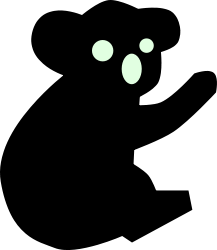
\includegraphics[height=1cm]{DarkKoala.png}}
\end{document}